% For VIM to recognize the document syntax \begin{document} and \end{document}
% - However, the compilation will fail!! So don't forget to comment the
%   directives before compiling!!'
%
%\begin{document}
%
% CHAPTER - Introduction -------------------------
\chapter{Introduction}%
\label{ch:introduction}
The present work illustrates the application of the two first stages of the Waterfall methodology
--- Analysis and Design --- to develop a \gls{tv} remote control. This type of project
begins with the establishment of a contract between the client (Samsung company)
and the project team, clearly defining the problem statement and deriving the
product requirements and constraints associated to the project. It should be
noted, however, that both roles are played out by the authors.
A market
research is performed to gain more insight over this market and the
product placement, and the product overall characteristics.

In the analysis
phase, the product requirements are derived --- defining the client expectations
for the product --- as well as the project constraints --- what the environments
limits about the product. Finally, the theoretical foundations are outlined,
providing the basic technical knowledge to undertake the project.

In the design phase, the product development starts, specifying the system in
terms of hardware and software and its associated interfaces, the error handling
required, and the design verification.
%
%  \vspace{-5mm}
  %
\section{Problem statement}%
\label{sec:prob-stat}
%The first step of the project is to clearly define the problem, as a result of
%the contract established between the client and the project team, yielding, in
%this case, the following project statement:
%
%``Design a remote control with three buttons that can
%remotely control the television (TV). It should be very
%light, powered by batteries and controls your TV via an
%infrared emitter. The TV has a built-in infrared receiver. A
%button on the remote control switches the TV on/off and
%will be labeled with the word "Power". The other two
%buttons are used to scroll up/down and select the available
%channels and they are labeled with the arrows up/down.''

%COVID pandemics presented a landmark on human interaction, greatly reducing the
%contact between people and surfaces. Thus, it is an imperative to provide people
%with contactless interfaces for everyday tasks. People redefined their
%purchasing behaviors, leading to a massive growth of the online
%shopping. However, some business sectors, like clothing or perfumes, cannot
%provide the same user experience when moving online.
%Therefore, one proposes to close that gap by providing a marketing digital
%outdoor for brands to advertise and gather customers with contactless
%interaction.
%
%Scenting marketing is a great approach to draw people into stores.
%Olfactory sense is the fastest way to the brain, thus, providing an exceptional
%opportunity for marketing~\cite{news-harvard} --- ``75\% of the emotions we generate on a daily basis are affected by smell. Next
%to sight, it is the most important sense we have''~\cite{lindstrom2006brand}.
%
%Combining that with additional stimuli, like sight and sound, can
%significantly boost the marketing outcome. Brands can buy advertisement space
%and time, selecting the videoclips to be displayed and the fragrance to be
%used at specific times, drawing the customers into their stores.
%
%Marketing also leverages from better user experience, thus, user interaction is
%a must-have, providing the opportunity to interact with the customer. In this
%sense, when users approach the outdoor a gesture-based interface will be
%provided for a brand immersive experience, where the user can take pictures or
%create GIFs with brand specific image filters and share them through their
%social media, with the opportunity to gain several benefits.

The first step of the project is to clearly define the problem, taking into
consideration the problem's context and motivation and exploiting the market opportunities.

\emph{The project consists of a \gls{mdo} with sound and
video display, and fragrance emission selected by the brands, providing a gesture-based interface for
user interaction to create pictures and \gls{gif}s, brand-specific, and share them on
social media.} It is comprised of several modes:
\begin{item-c}
\item \emph{normal mode (advertisement mode)}: the \gls{mdo} will provide
  sound, video and fragrance outputs.
\item \emph{interaction mode}: When a user approaches, the \gls{mdo} it will
go into interaction mode, turning on and displaying the camera feed and waiting
for recognizable gestures to provide additional functionalities, such as
brand-specific image filters.
\item \emph{sharing mode}: after a user take a picture or create a \gls{gif}, it
  can share it across social media.
\end{item-c}

Brands can buy advertisement space and time, selecting the videoclips to be
displayed and the fragrance to be used at specific times, drawing the customers
into their stores. Customers can be captivated by the combination of sensorial
stimuli, the gesture-based interaction, the immersive user experience provided
by the brands --- feeling they belong in a TV advertisement, and the opportunity
to gain several benefits, e.g., discount coupons.
%%% Local Variables:
%%% mode: latex
%%% TeX-master: "../../../dissertation"
%%% End:

\section{Context and motivation}
\label{sec:context-motivation}


%%% Local Variables:
%%% mode: latex
%%% TeX-master: "../../../dissertation"
%%% End:

\section{Market research}
\label{sec:market-research}
A Digital Outdoor is essentially a traditional outdoor advertising powered up by technology. 
The pros of a digital outdoor compared to a traditional one is mostly the way that it captivates the attention of consumers in a more dynamic way. 
It can also change its advertisement according to certain conditions, such as
weather and/or time. Some researches tells that the British public sees over 1.1
\gls{bn} digital outdoor advertisements over a week~\cite{digital-outdoor}, which can tell how much digital marketing is valued nowadays.

When talking about numbers, ``At the end of 2020, despite the Covid wipeout, the \gls{dooh} market was estimated to be worth \$41.06 \gls{bn}, but by 2026, nearly two out of three (65\%) advertising executives predict this will rise to between \$50 \gls{bn} and \$55 \gls{bn}. 
A further 16\% expect it to be worth between \$55 \gls{bn} and \$60 \gls{bn}, and 14\% estimate it will be even bigger''~\cite{outdoor-market}.

\begin{figure}[htb!]
\centering
    
\includegraphics[width=0.7\columnwidth]{./img/DigitalOutdoor.png}
  \caption{Example of a Digital Outdoor, withdrawn from~\cite{digital-outdoor}}%
\label{fig:dig-outdoor}
\end{figure}

Scent market is the art of taking a company's brand identity, marketing messages, target audience and creating a scent that amplifies these values. 
That's because ``a scent has the ability to influence behavior and trigger memories almost instantaneously. When smell is combined with other marketing cues, it can amplify a brand experience and establish a long lasting connection with consumers''~\cite{scent-market}.

Ambient scent uses fragrance to enhance the experience of consumers with different purposes, whereas scents in scent branding are unique to each company's identity.
According to a Samsung study: ``when consumers were exposed to a company scent, shopping time was increased by 26\% and they visited three times more product categories'' ~\cite{scent-stats}.
Also, ``the digital scent technology market is expected to grow from \$1.0 \gls{bn} in 2021 to \$1.5 \gls{bn} by 2026, at a \gls{cagr} of 9.2\%.''~\cite{scent-money}.

\begin{figure}[htb!]
\centering
    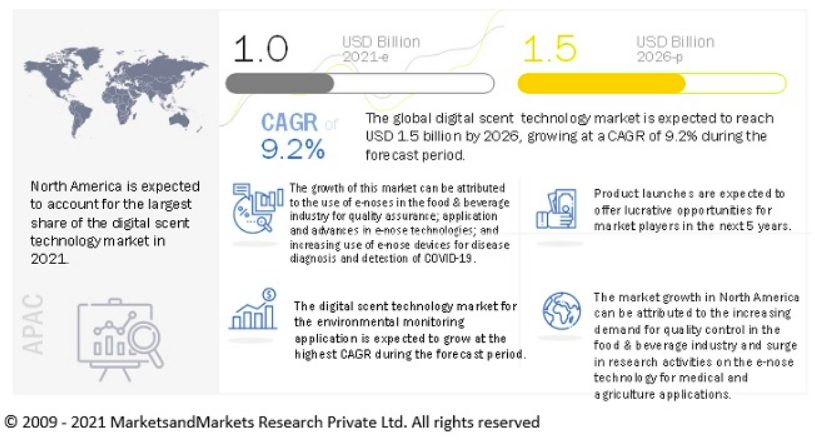
\includegraphics[width=0.9\columnwidth]{./img/scentstats.png}
  \caption{Attractive Opportunities in the Digital Scent Technology Market, withdrawn from~\cite{scent-money}}%
\label{fig:scent-stat}
\end{figure}

The market growth can be attributed to several factors, such as expanding application and advancements in e-nose technologies, increasing use of e-nose devices for disease diagnostic applications, emerging \gls{rd} activities to invent e-nose to sniff out COVID-19, and rising use of e-nose in food industry for quality assurance in production, storage, and display.

% Remote material (side by side)
%\begin{figure}[htb!]
%  \centering
  %
%  \begin{subfigure}{.4\textwidth}
%  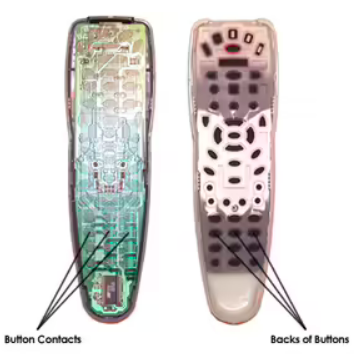
\includegraphics[width=\textwidth]{img/remotematerial1.png}%
  %\caption{KUKA's original position}%
  %\label{fig:ptp-test-orig}
%\end{subfigure}
%
 % \begin{subfigure}{.4\textwidth}
  %  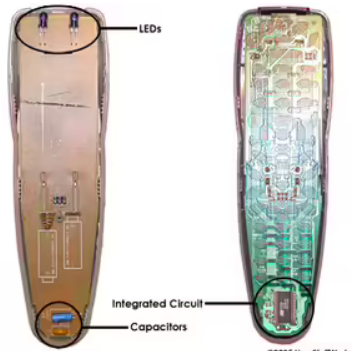
\includegraphics[width=\textwidth]{img/remotematerial2.png}%
%  \caption{KUKA's final position}%
%  \label{fig:ptp-test-final}
%\end{subfigure}
%
%  \caption{TV Remote control bill of materials, withdrawn from~\cite{remotematerial}}%
%  \label{fig:remotemat}
%\end{figure}
%

%%% Local Variables:
%%% mode: latex
%%% TeX-master: "../../../dissertation"
%%% End:

\section{Project goals}%
\label{sec:project-goals}
The project aims to develop a \gls{cps} for multi-sensorial marketing with
contactless user interaction. The key goals identified and the respective path
to attain them are:
\begin{enum-c}
\item \emph{devise a device with audio and video outputs, as well as fragrance
    diffusion}: understand audio and video streaming and study fragrance
  nebulizer technologies.
\item \emph{create a contactless user interface based on gestures through
    computer vision}: identify user gestures through computer vision and match them to interface
  callbacks; a virtual keyboard may be required for user input.
\item \emph{devise a distributed architecture to convey brand advertisement
  information to the local device}: understand distributed architectures and
apply them for optimal data flow; create a remote client-server model to convey
information from the brands to the device through remote cloud database
services; devise adequate data frames to convey information to the local device;
create a local server to respond to the remote server requests.
\item \emph{apply facial recognition to the camera feed and subsequently apply
  image filters specific to each brand}: understand facial recognition
algorithms and apply them to the camera feed; apply image filters on top of the
identified faces through a specialized \gls{api}.
\item \emph{enable image and GIFs sharing to social media for increased brand
    awareness}: understand how to use social media APIs for media sharing.
\end{enum-c}
%
%%% Local Variables:
%%% mode: latex
%%% TeX-master: "../../../dissertation"
%%% End:

\section{Report Outline}
\label{sec:report-outline}
This report is organised as follows:
\begin{itemize}
%\item In Chapter~\ref{ch:state-art}, the state of the art of remote controlled
%vehicles is presented.
%\item In Chapter~\ref{ch:theor-found} lays out the theoretical foundations for
%  project development,
%  namely the project development methodologies and associated tools, and the
%  communications technologies.
%\item In Chapter~\ref{ch:requirements-specs} are identified the key requirements
%  and constraints the system being developed must meet from the end-user
%  perspective (requirements) and, by defining well-established boundaries within
%  the project resources (time, budget, technologies and know-how), the list of
%  spefications is obtained.
%\item After defining the product specifications, the solutions space is explored
%  in Chapter~\ref{ch:analysis}, providing the rationale for viable solutions and
%  guiding the designer towards a best-compromise solution, yielding the
%  preliminary design and the foreseen tests to the specifications.
%\item The preliminary design is further refined in Chapter~\ref{ch:design} and
%  decomposed into tractable blocks (subsystems) which can be designed
%  independently and assigned to different design teams, allowing the transition
%  to the implementation phase.
%\item Next, in Chapter~\ref{ch:implementation}, the design solution is
%  implemented into the target platforms.
%\item Then, in Chapter~\ref{ch:testing}, the implementation is tested at the
%  subsystem level (unit testing) and system level (integrated testing),
%  analysing and comparing the attained performance with the expected one.
%\item After product testing, in Chapter~\ref{ch:verif-valid}, the specifications
%  must be verified and validated by an external agent.
%  subsystem level (unit testing) and system level (integrated testing),
%  analysing and comparing the attained performance with the expected one.
%\item Chapter~\ref{ch:conclusion} gives a summary of this report as well as
%  prospect for future work.
\item Lastly, the appendices (see Section~\ref{ch:Append}) contain detailed
  information about project planning and development.
\end{itemize}


%%% Local Variables:
%%% mode: latex
%%% TeX-master: "../../../dissertation"
%%% End:

%
%%% Local Variables:
%%% mode: latex
%%% TeX-master: "../../../dissertation"
%%% End:
